
The performance of the axiom weakening base repair algorithm shown in \cref{algo:repair-weaken} has also been evaluated. During each repair via axiom weakening, the time taken and the number of calls to the reasoner have been registered. Additionally, the number of steps taken by the repair using axiom weakening has been observed. Also, as mentioned in \cref{eval-quality}, the repair program was put under a timeout to prevent cases where the reasoning becomes unreasonably slow. The generation of inconsistent ontologies used a similar timeout and the same procedure was used for situations in which the reasoner ran out of memory. Timeout of the weakening procedure are shown separately from those latter cases in the results. The frequency of these cases is indicated as percentage of the overall runs finished vs started. The results of this evaluation are presented in \cref{table:results-perf}, \cref{fig:results-perf-calls} and \cref{fig:results-perf-time}.

\begin{table}[ht]
  \scriptsize
  \centering
  \begin{tabular}{|l|cccc|}
    \hline
    & Steps & Calls & Time [ms] & Failed \\
    \hline
    admin & 8.5 & 9462 & 15649 & 01\% (01\%) \\
    ahso & 2.1 & 4783 & 11922 & 10\% (28\%) \\
    cdao & 2.4 & 16734 & 20674 & 12\% (47\%) \\
    cdpeo & 1.6 & 4633 & 2068 & 00\% (00\%) \\
    covid19-ibo & 1.3 & 14632 & 2186 & 04\% (12\%) \\
    ecp & 1.3 & 2027 & 6034 & 00\% (12\%) \\
    emo & 1.5 & 19013 & 5624 & 00\% (02\%) \\
    evi & 5.5 & 6405 & 4916 & 10\% (68\%) \\
    falls & 1.6 & 1328 & 876 & 02\% (07\%) \\
    fo & 1.5 & 1282 & 1064 & 25\% (62\%) \\
    gbm & 1.5 & 8092 & 2911 & 00\% (00\%) \\
    gfvo & 1.8 & 4199 & 2352 & 00\% (00\%) \\
    koro & 1.8 & 6340 & 2277 & 00\% (00\%) \\
    lico & 2.7 & 7013 & 3661 & 01\% (20\%) \\
    mamo & 2.6 & 4799 & 2243 & 00\% (00\%) \\
    mpio & 2.4 & 1987 & 999 & 08\% (30\%) \\
    pizza & 2.0 & 7453 & 28225 & 19\% (57\%) \\
    provo & 5.0 & 7000 & 8587 & 05\% (10\%) \\
    qudt & 1.1 & 7150 & 6389 & 08\% (41\%) \\
    trans & 1.7 & 3218 & 1494 & 00\% (06\%) \\
    triage & 2.4 & 4295 & 6107 & 17\% (49\%) \\
    vio & 2.7 & 9406 & 10955 & 04\% (07\%) \\
    \hline
  \end{tabular}
  \caption{Results of the evaluation with respect to performance. Number of weakening iterations, reasoner calls, and total repair time are given as sample mean, with 95\% confidence interval in brackets. The frequency of failed runs is shown as percentage of repairs by weakening that were started but not completed. In parentheses the percentage of total failed runs including those with timeout during generation of inconsistent ontologies.}
  \label{table:results-perf}
\end{table}

\begin{figure}[ht]
  \centering
  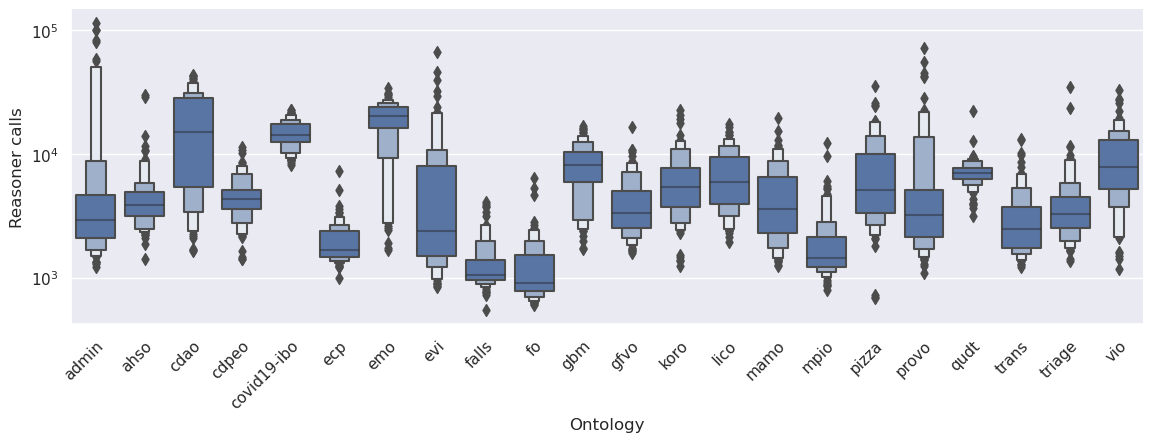
\includegraphics[width=\textwidth]{resources/calls-ontology-violin.png}
  \caption{Distribution of reasoner calls required for repairing a single ontology using axiom weakening. Attempts that failed by timeout or other errors were not considered.}
  \label{fig:results-perf-calls}
\end{figure}

\begin{figure}[ht]
  \centering
  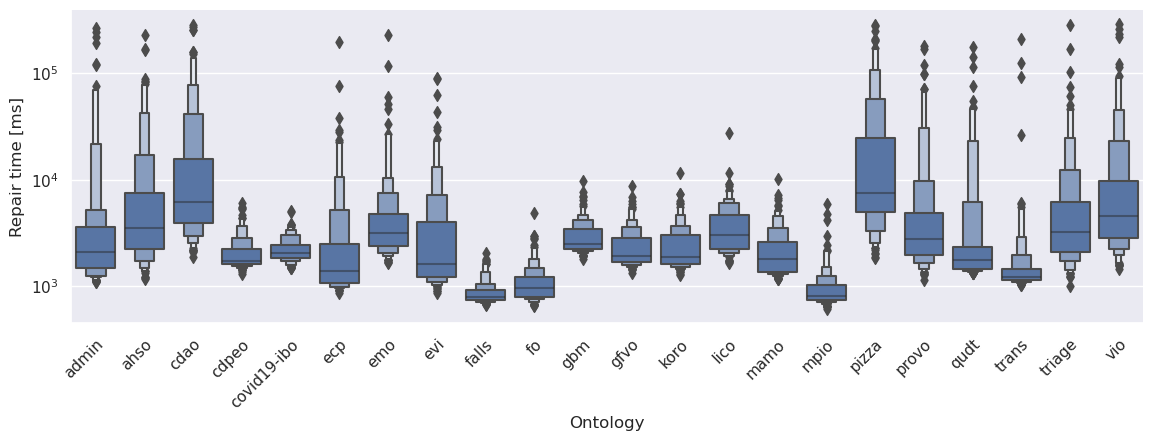
\includegraphics[width=\textwidth]{resources/time-ontology-violin.png}
  \caption{Distribution of (real) execution time required for repairing a single ontology using axiom weakening. Attempts that failed by timeout or other errors were not considered.}
  \label{fig:results-perf-time}
\end{figure}

As is visible from the results, the number of reasoner calls and the execution time can vary significantly. The execution times were generally reasonable when a run was able to complete within the time limit, with most of them completing within 2 minutes, even though the time limit was set to 5 minutes. A significant number of runs, however, was affected by the timeout or other errors. It has not been looked deeper into what causes these issues.

